\documentclass[border=5pt]{standalone}
\usepackage{fontspec,unicode-math}
\setmainfont{Noto Serif}
\setmathfont{STIXTwoMath-Regular.otf}
\usepackage{tikz}
\usetikzlibrary{arrows.meta,calc,patterns,decorations.markings}
\definecolor{Ink}{HTML}{000000}
\tikzset{ax/.style={draw=Ink,line width=.65pt,-{Latex[length=2.2mm,width=1.25mm]}},
lev/.style={draw=Ink,line width=1.25pt,line cap=butt},
fine/.style={draw=Ink,line width=.60pt},
band/.style={draw=Ink,line width=.62pt},
sol/.style={draw=Ink,line width=1.35pt,line cap=round,line join=round},
ray/.style={draw=Ink,line width=.72pt,-{Latex[length=2.0mm,width=1.15mm]}},
dim/.style={draw=Ink,line width=.60pt,{Latex[length=1.7mm,width=.95mm]}-{Latex[length=1.7mm,width=.95mm]}},
lab/.style={text=Ink,font=\fontsize{13}{16}\selectfont,inner sep=1.1pt},
small/.style={text=Ink,font=\fontsize{11}{13}\selectfont,inner sep=1.0pt}}
\pagestyle{empty}
\def\datadir{data}
\IfFileExists{data/F20_1_heat.dat}{}{\def\datadir{../data}}
\begin{document}
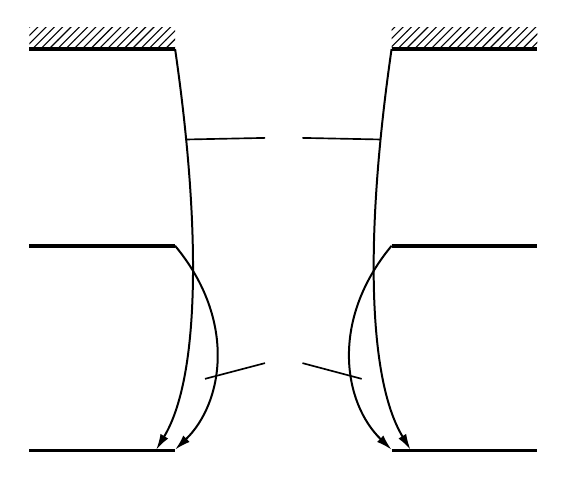
\begin{tikzpicture}[x=1cm,y=1cm]

\foreach \x in {.5,5.1}{
 \draw[lev] (\x,.5)--++(1.85,0) (\x,3.1)--++(1.85,0) (\x,5.6)--++(1.85,0);
 \fill[pattern=north east lines,pattern color=Ink] (\x,5.62) rectangle ++(1.85,.25);
}
\draw[ray] (2.35,5.60) .. controls (2.67,3.40) and (2.68,1.45) .. (2.11,.51);
\draw[ray] (5.10,5.60) .. controls (4.78,3.40) and (4.77,1.45) .. (5.34,.51);
\draw[ray] (2.35,3.10) .. controls (3.14,2.15) and (2.96,1.10) .. (2.35,.51);
\draw[ray] (5.10,3.10) .. controls (4.31,2.15) and (4.49,1.10) .. (5.10,.51);
\node[lab] (charge) at (3.73,4.47) {РПЗ};
\draw[fine] (charge.west)--(2.50,4.45) (charge.east)--(4.96,4.45);
\node[lab] (exc) at (3.73,1.61) {РПВ};
\draw[fine] (exc.west)--(2.73,1.41) (exc.east)--(4.72,1.41);
\end{tikzpicture}
\end{document}
